\begin{figure}[H]%
	\ThisCenterWallPaper{1}{images/\texorpdfstring{\chaptername\thechapter}}%
	\captionlistentry[figure]{Icon of \chaptername\ \thechapter}% figure with chapter and section number
	%\addcontentsline{lof}{figure}{Icon of \chaptername\ \thechapter}% figure without chapter and section number
	\label{fig:\chaptername\thechapter}%
\end{figure}

\vspace*{-4.3cm}
\epigraph{"We at Google have made tremendous advances in understanding language. Our knowledge graph has been fundamental to that..."}{\textit{--- Amit Singhal}}

\noindent \large{\textbf{This {\MakeLowercase{\chaptername}}'s contents:}}
\vspace*{-1.0cm}
\minitoc \mtcskip \minilof
\vspace*{-0.5cm}

In this chapter are presented the results post implementation of the WebApp.
\vspace*{-0.25cm}

\section{Frontend search form} \label{section:Displayoftheresults/Frontendsearchform}
This first section is about the searching of a start vertex from the user inputting node names or titles and the number of hops from that vertex to all the other vertices that shall be shown in the graph.

In \hyperref[fig:SnapshotSearchFormGargantini]{\autoref{fig:SnapshotSearchFormGargantini}} is displayed the search process of a node, in the specific case of the name of professor Gargantini, University of Bergamo.

\begin{figure}[H]%
	\centering%
	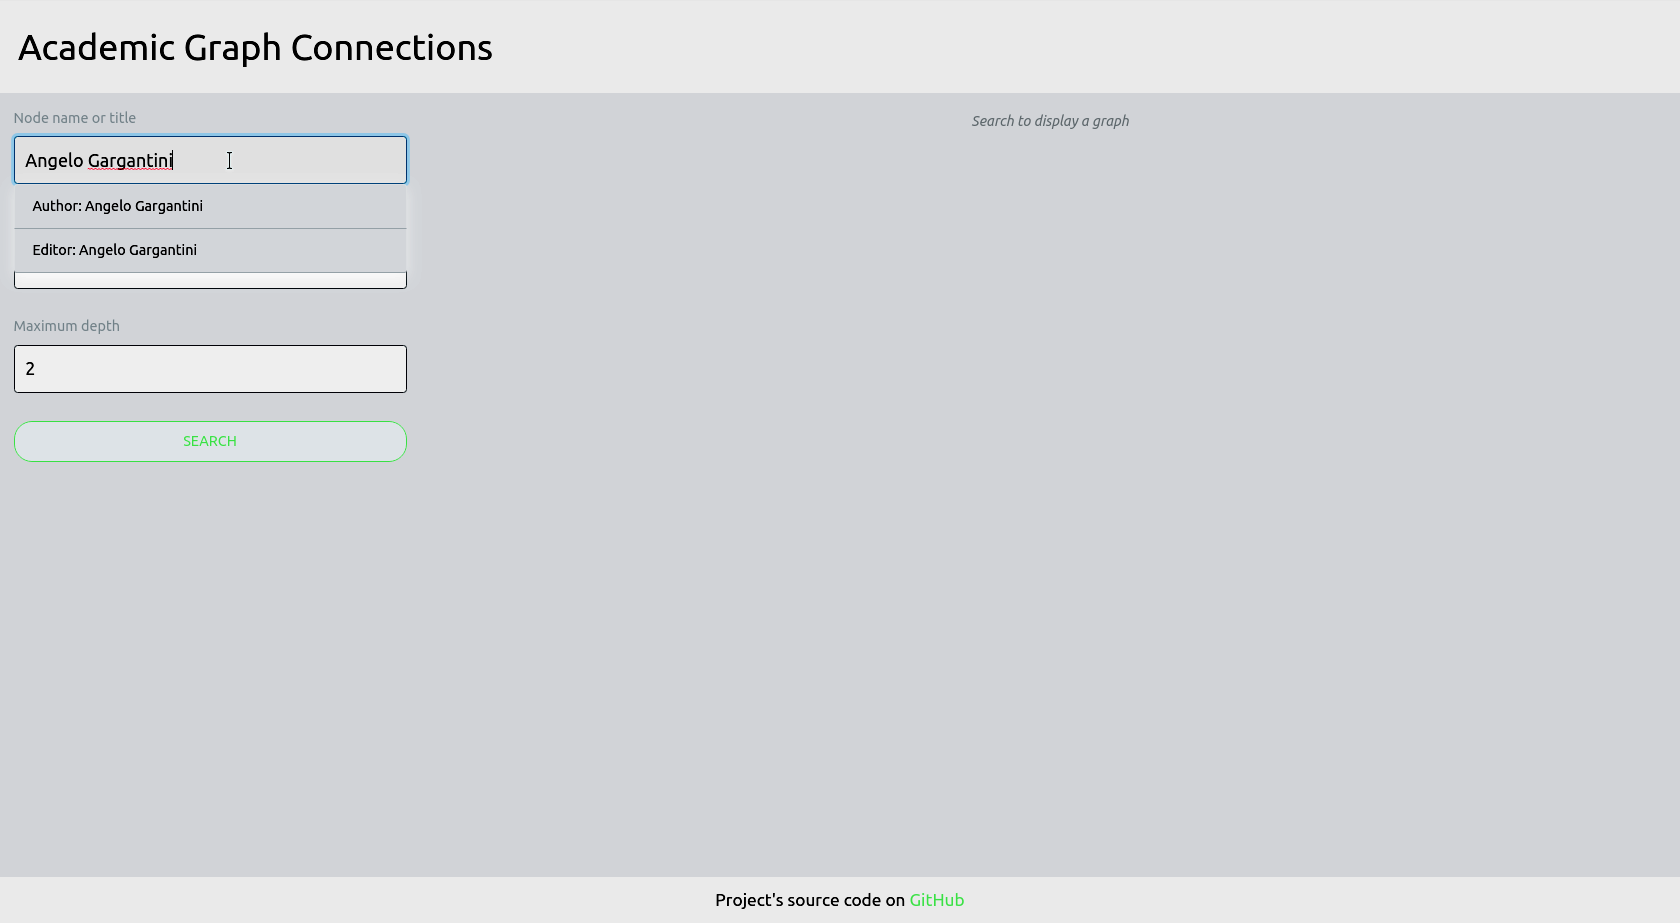
\includegraphics[%
		width=1\textwidth-4pt,%
		bgcolor=white,%
		cfbox=lightestgray % color
			  2pt % rule width
			  0pt % rule separation
			  0pt % margin
	]{images/chapter5/SnapshotSearchFormGargantini.png}%
	\caption[Searching for a vertex named "Angelo Gargantini", selecting the element from the suggested list]{Searching for a vertex named "Angelo Gargantini", selecting the element from the suggested list}%
	\label{fig:SnapshotSearchFormGargantini}%
\end{figure}%

The user inputs a string and in a moment a suggestion list of nodes with that name or title pops up.
Supposing to have selected the author element of the pop up list, it is possible to input the values for the other two fields of the search form.

By default are set to 1 and 2 the number of hops, that is the minimum depth and maximum depth. These values indicate the distance from the start node (chosen in the first field of the search form) of the vertices to be included in the graph.

In \hyperref[fig:SnapshotLoadingGraphGargantini]{\autoref{fig:SnapshotLoadingGraphGargantini}} is visualized the webpage just after having clicked on the search button. At this precise moment the \gls{GraphQL} \acrshort{API} is queried and the database is performing the needed calculations.

\begin{figure}[H]%
	\centering%
	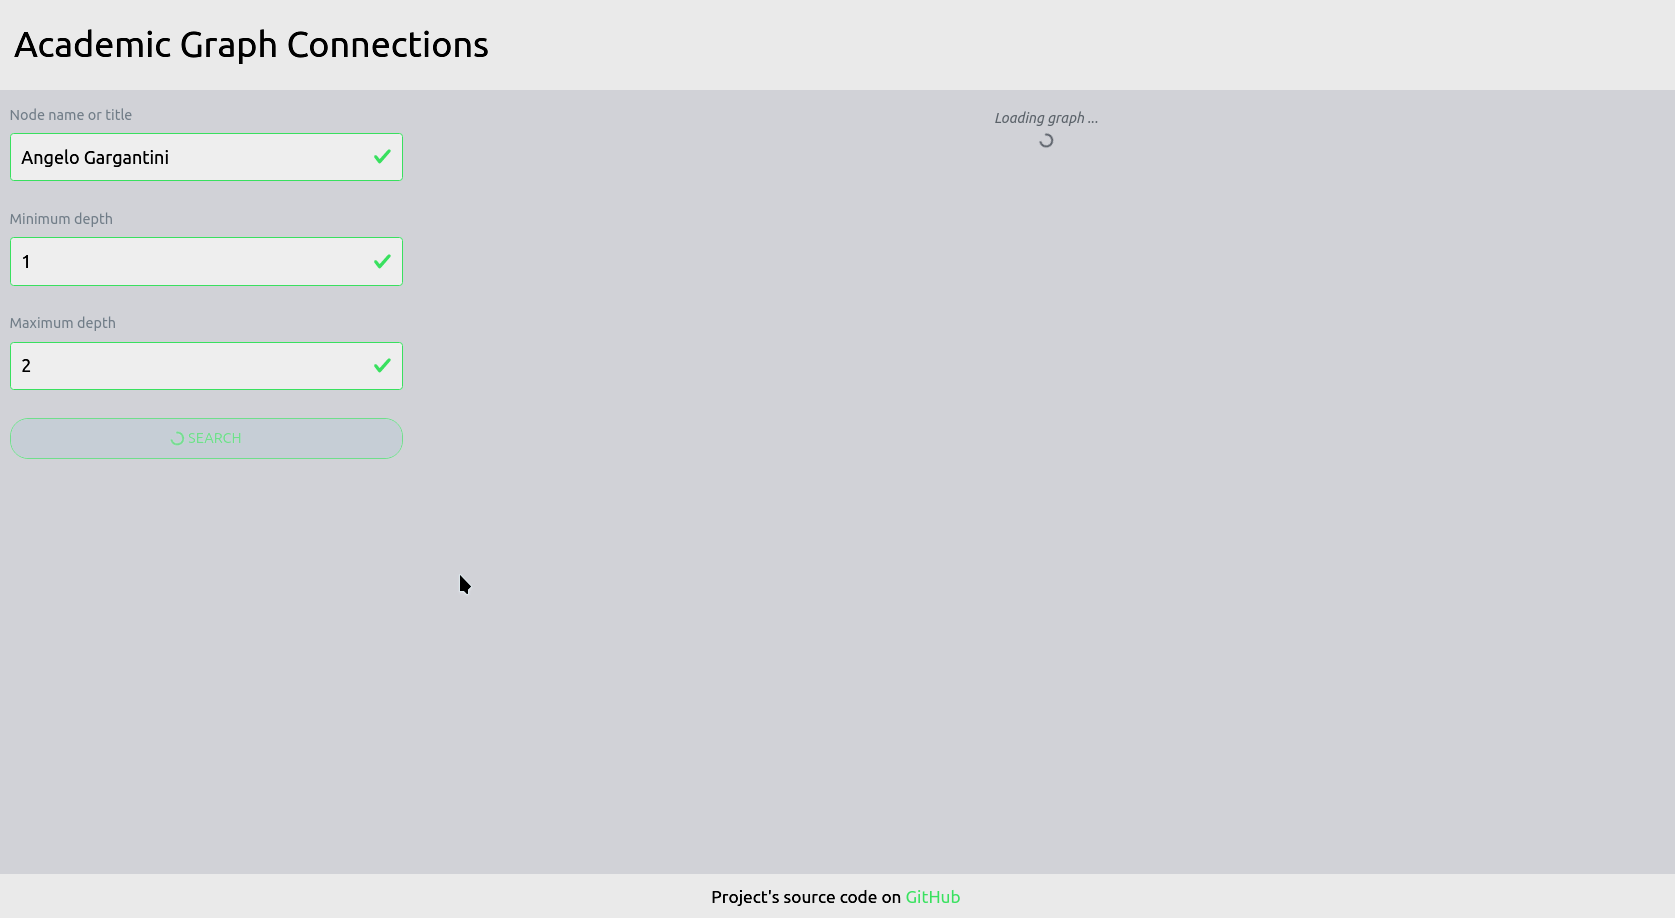
\includegraphics[%
		width=1\textwidth-4pt,%
		bgcolor=white,%
		cfbox=lightestgray % color
			  2pt % rule width
			  0pt % rule separation
			  0pt % margin
	]{images/chapter5/SnapshotLoadingGraphGargantini.png}%
	\caption[Collaboration graph of prof. Gargantini loading]{Collaboration graph of prof. Gargantini loading}%
	\label{fig:SnapshotLoadingGraphGargantini}%
\end{figure}%

In the next section the loading graph's results are visualized.
The results are limited to just a frontend, client interface point of view since that is the main usecase of the developed \gls{WebApp}.
What happens behind the scenes with the querying and the traversal computation to show the results, is not treated here.
For a more detailed explanation of how everything is integrated together see \hyperref[chapter:CommunityDetection]{\S\ \ref{chapter:CommunityDetection} - \nameref{chapter:CommunityDetection}} on \hyperref[chapter:CommunityDetection]{page \pageref*{chapter:CommunityDetection}} and  \hyperref[chapter:ImplementingtheWebApp]{\S\ \ref{chapter:ImplementingtheWebApp} - \nameref{chapter:ImplementingtheWebApp}} on \hyperref[chapter:ImplementingtheWebApp]{page \pageref*{chapter:ImplementingtheWebApp}}.

\section{Frontend graph visualization} \label{section:Displayoftheresults/Frontendgraphvisualization}
Once the database has traversed the graph from the start vertex to all the other nodes at distance 1 to 2, the list of the visited nodes, of the edges connecting them and of their communities gets sent back from the \acrshort{API} to the frontend.
The graph rendering libraries use this data to fit all the nodes in a canvas for the user to easily navigate on.

In \hyperref[fig:SnapshotLoadedGraphGargantini]{\autoref{fig:SnapshotLoadedGraphGargantini}} (and in \hyperref[fig:SnapshotLoadedGraphGargantiniCut]{\autoref{fig:SnapshotLoadedGraphGargantiniCut}} focused on the canvas) is rendered the collaboration graph searched for, with the detected collaboration communities highlighted in rectangular compound nodes.

There are many communities shown because some of the researchers with whom prof. Gargantini has collaborated are more tightly connected to other groups of researchers, which means they belong to some other collaboration community.

Some communities are displayed having only one node. This happens because many of the other nodes of those communities are not in the range 1 to 2 - minimum and maximum depth, distance from the start node that was searched at the beginning in the shown example. While it makes sense from the theoretical point of view to have 1-member communities, this is not what is happening in this case.

\begin{figure}[H]%
	\centering%
	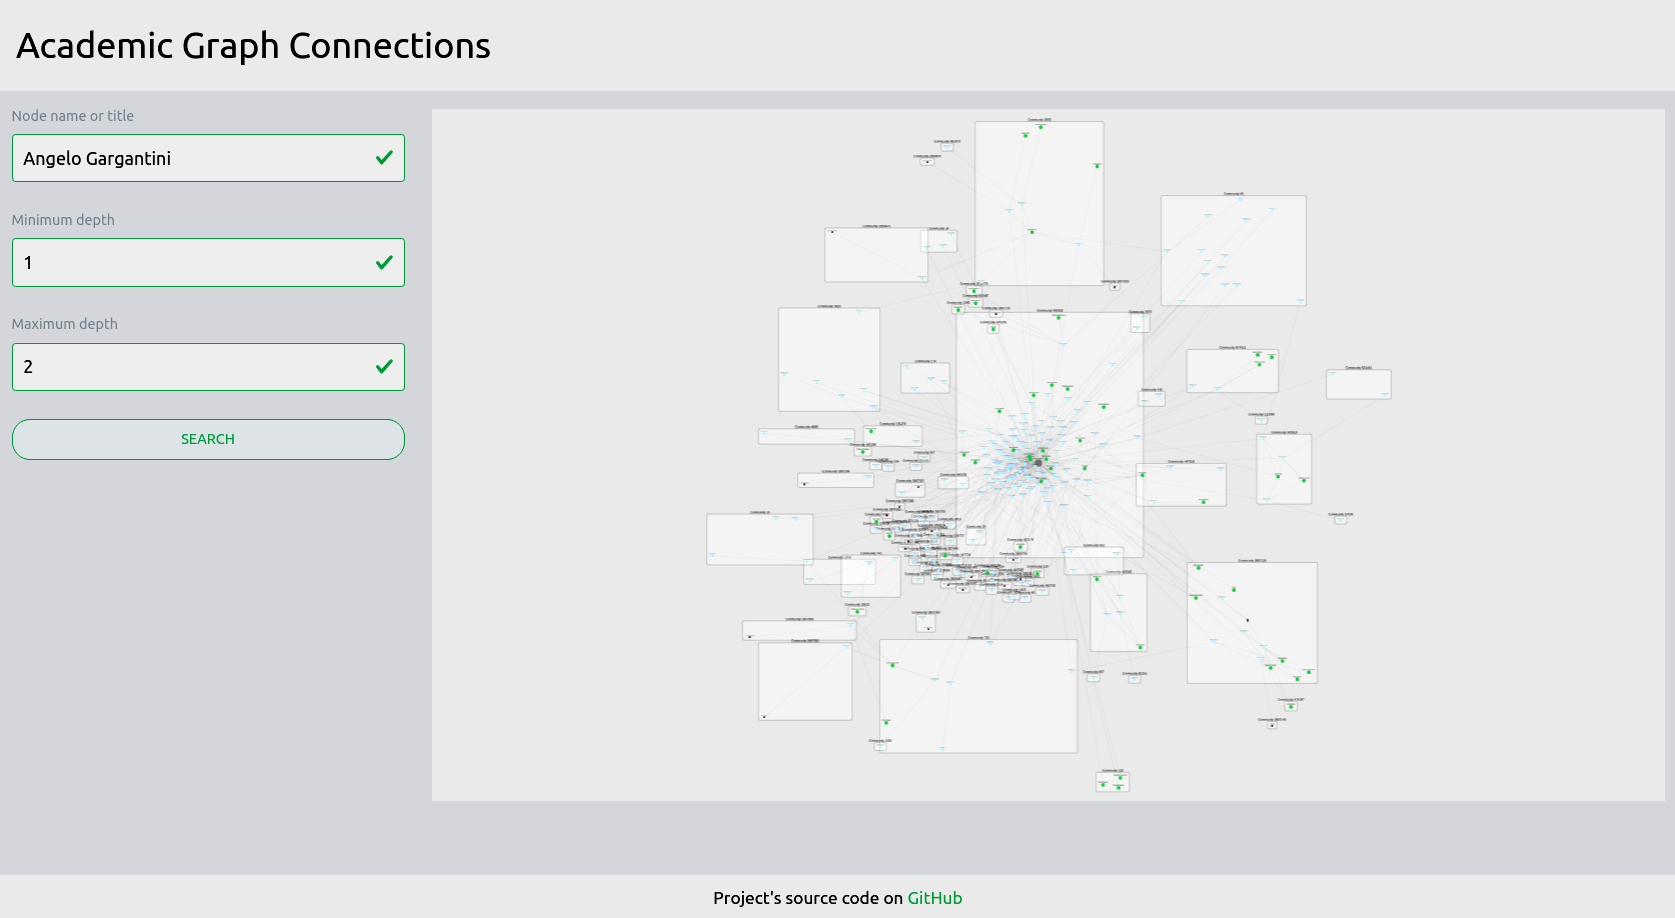
\includegraphics[%
		width=1\textwidth-4pt,%
		bgcolor=white,%
		cfbox=lightestgray % color
			  2pt % rule width
			  0pt % rule separation
			  0pt % margin
	]{images/chapter5/SnapshotLoadedGraphGargantini.png}%
	\caption[Visualizing the collaboration graph in the WebApp]{Visualizing the collaboration graph in the \gls{WebApp}}%
	\label{fig:SnapshotLoadedGraphGargantini}%
\end{figure}%

A consideration worthy to be made, in view of possible improvements treated in \hyperref[subsection:Conclusions/Possibleimprovements/Collapsibleandexpandablecommunitycompoundnodes]{\S\ \ref{subsection:Conclusions/Possibleimprovements/Collapsibleandexpandablecommunitycompoundnodes}} on \hyperref[subsection:Conclusions/Possibleimprovements/Collapsibleandexpandablecommunitycompoundnodes]{page \pageref{subsection:Conclusions/Possibleimprovements/Collapsibleandexpandablecommunitycompoundnodes}} - is the possibility of having the compound nodes (community nodes), collapsible and expandable.\label{tobementionedinconclusions/Collapsibleandexpandablecommunitycompoundnodes}

\begin{figure}[H]%
	\centering%
	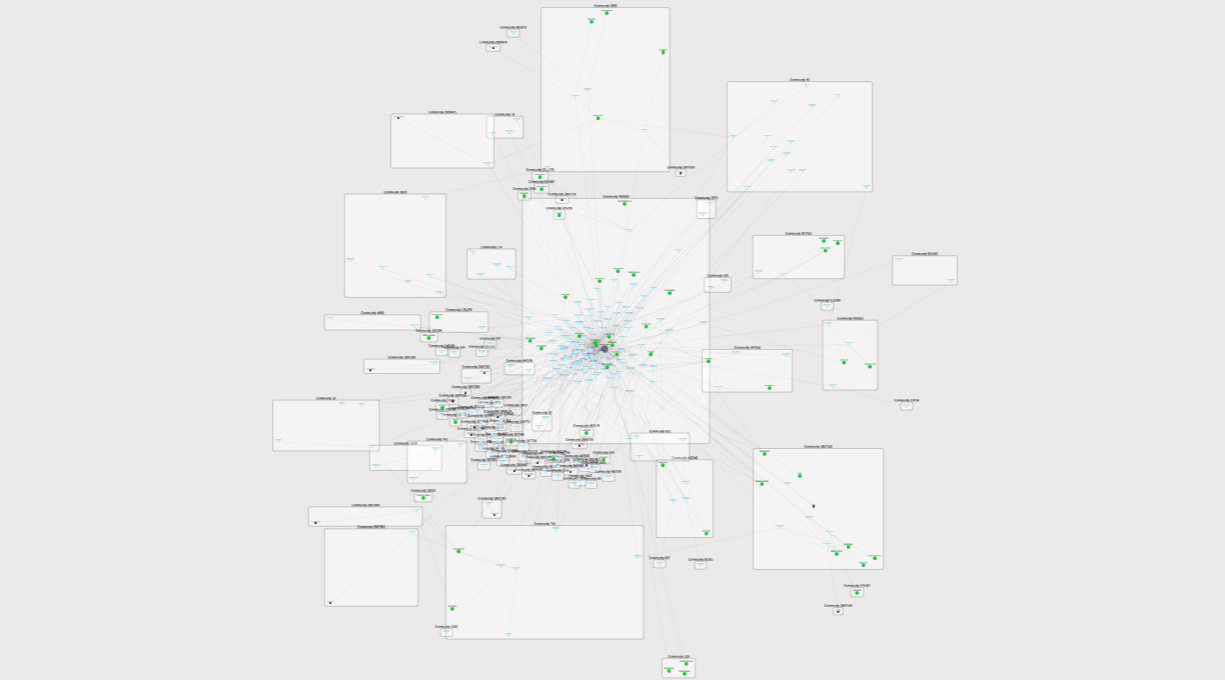
\includegraphics[%
		width=1\textwidth-4pt,%
		bgcolor=white,%
		cfbox=lightestgray % color
			  2pt % rule width
			  0pt % rule separation
			  0pt % margin
	]{images/chapter5/SnapshotLoadedGraphGargantiniCut.png}%
	\caption[Plain view of the canvas where the graph is rendered]{Plain view of the canvas where the graph is rendered}%
	\label{fig:SnapshotLoadedGraphGargantiniCut}%
\end{figure}%

In the next section detail level zoomed graphs are shown and their features are interpreted.

\section{Detailed view of some examples of graphs of collaboration communities} \label{section:Displayoftheresults/Detailedviewofsomeexamplesofgraphsofcollaborationcommunities}

\subsection{Prof. Angelo Gargantini's cluster of research collaboration} \label{subsection:Displayoftheresults/Indetailviewofthecollaborationgraph/ProfAngeloGargantinisclusterofresearchcollaboration}
\begin{figure}[H]%
	\centering%
	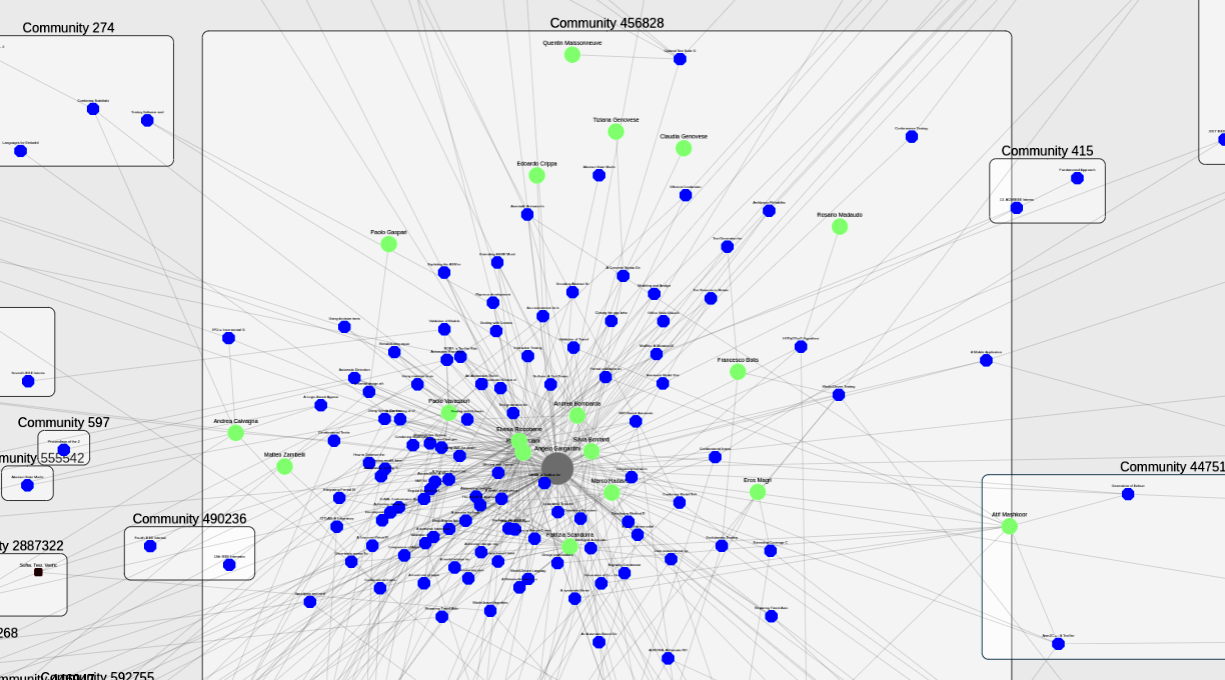
\includegraphics[%
		width=1\textwidth-4pt,%
		bgcolor=white,%
		cfbox=lightestgray % color
			  2pt % rule width
			  0pt % rule separation
			  0pt % margin
	]{images/chapter5/SnapshotLoadedGraphGargantiniZoom.png}%
	\caption[A zoomed view of the research collaboration community of prof. Gargantini]{A zoomed view of the reasearch collaboration community of prof. Gargantini}%
	\label{fig:SnapshotLoadedGraphGargantiniZoom}%
\end{figure}%

In the last searched graph, zooming in again in the middle where the start node is placed (author: Angelo Gargantini) - like in \hyperref[fig:SnapshotLoadedGraphGargantiniZoom]{\autoref{fig:SnapshotLoadedGraphGargantiniZoom}}, it is possible to see the dense relations (edges) between the vertices.
The dark blue nodes are publication works, while the light green ones are other peer researchers.

This panoramic is interesting because it makes it possible to grasp a sense of boundary of the community even without the rectangle highlighting it.
The transition from densely to sparsely linked is noticeable around the main group of nodes. The further is gone from its gravity center, the fewer the number of connections (edges) between this group's nodes and the others around it.

Zooming in again, this time to a level of detail able to read the names of the nodes like in \hyperref[fig:SnapshotLoadedGraphGargantiniZoomMore]{\autoref{fig:SnapshotLoadedGraphGargantiniZoomMore}}, some other considerations can be made. It is possible to see that some of the most tightly linked nodes of prof. Gargantini are indeed his real life collaborators, like his PhD students or his university colleagues, professors.

In the next subsection is considered one of the nodes that appeared in prof. Gargantini's collaboration graph, his colleague prof. Patrizia Scandurra.

\begin{figure}[H]%
	\centering%
	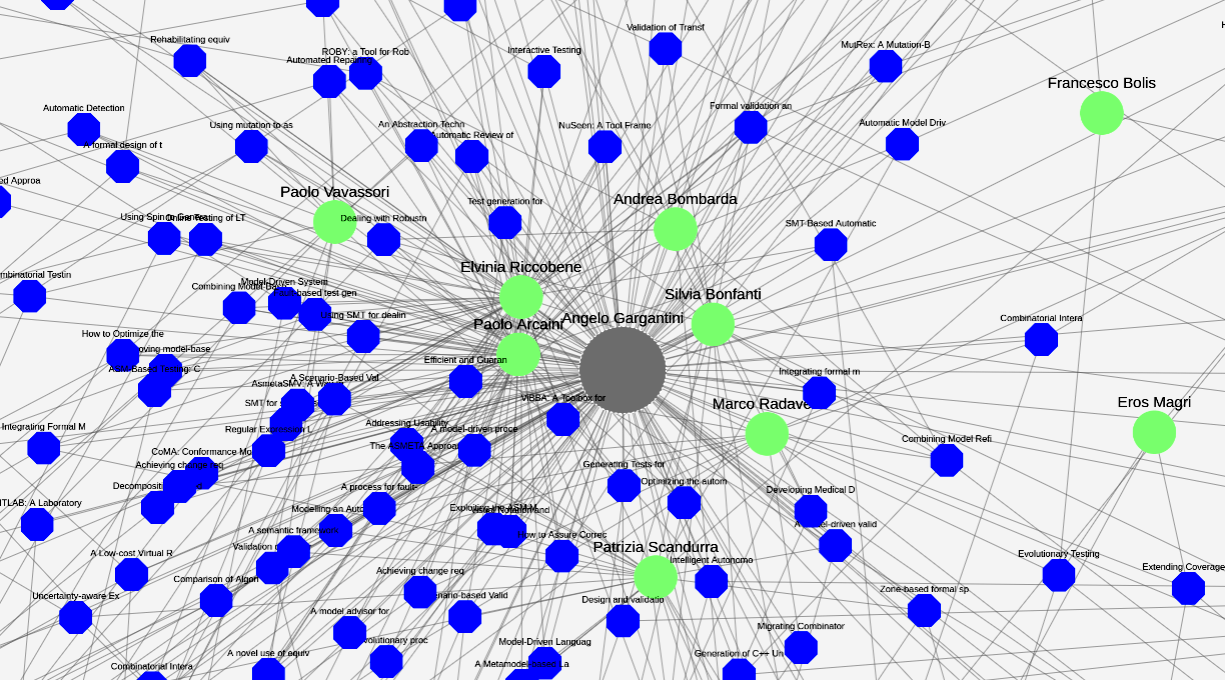
\includegraphics[%
		width=1\textwidth-4pt,%
		bgcolor=white,%
		cfbox=lightestgray % color
			  2pt % rule width
			  0pt % rule separation
			  0pt % margin
	]{images/chapter5/SnapshotLoadedGraphGargantiniZoomMore.png}%
	\caption[Detail level zoom of the collaboration graph of prof. Gargantini and its peers, publications]{Detail level zoom of the collaboration graph of prof. Gargantini and its peers, related publications}%
	\label{fig:SnapshotLoadedGraphGargantiniZoomMore}%
\end{figure}%

\subsection{Prof. Patrizia Scandurra's research collaboration cluster} \label{subsection:Displayoftheresults/Indetailviewofthecollaborationgraph/ProfPatriziaScandurrasresearchcollaborationcluster}
After having searched for the graph of prof. Scandurra, the zoomed view is the one shown in \hyperref[fig:SnapshotLoadedGraphScandurraZoomMore]{\autoref{fig:SnapshotLoadedGraphScandurraZoomMore}}.
As expected, since prof. Scandurra appeared in prof. Gargantini's collaboration community graph, also the viceverca is true.

\begin{figure}[H]%
	\centering%
	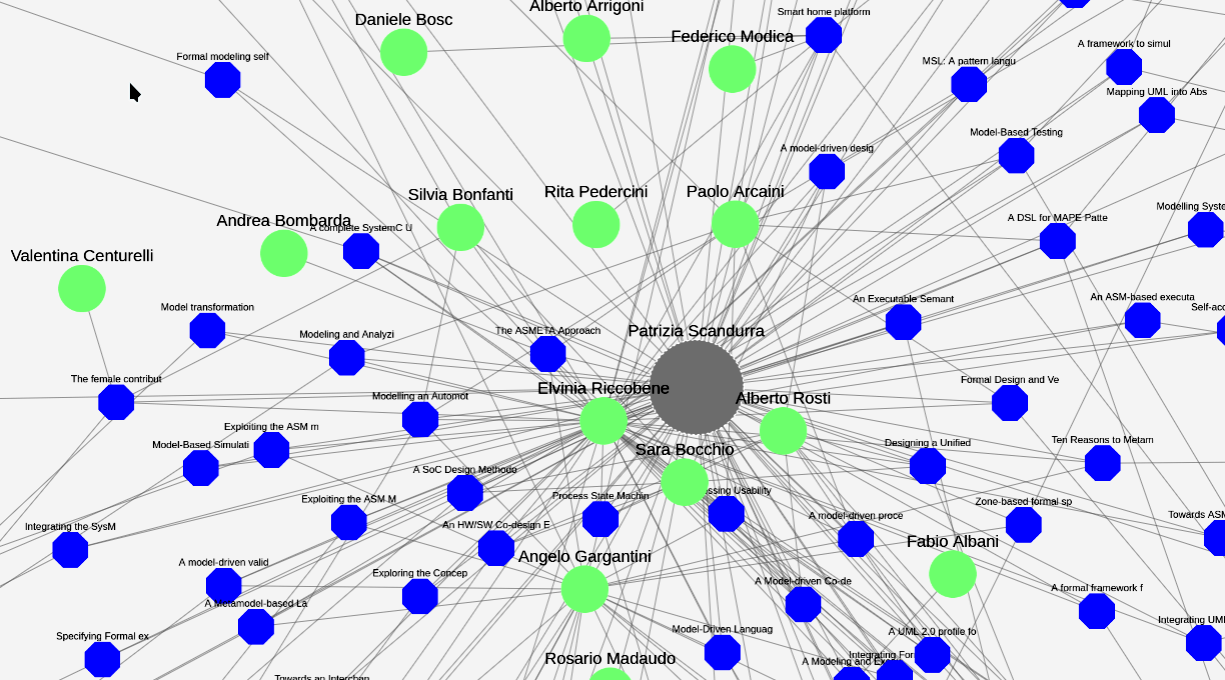
\includegraphics[%
		width=1\textwidth-4pt,%
		bgcolor=white,%
		cfbox=lightestgray % color
			  2pt % rule width
			  0pt % rule separation
			  0pt % margin
	]{images/chapter5/SnapshotLoadedGraphScandurraZoomMore.png}%
	\caption[Detailed view of the collaboration graph of prof. Scandurra and of its peers, publications]{Detailed view of the collaboration graph of prof. Scandurra and of its peers, publications}%
	\label{fig:SnapshotLoadedGraphScandurraZoomMore}%
\end{figure}%

Furthermore, both of them have many researchers in common in their research collaboration graphs.
In a sense, collaborating together and having many connections in common leads to being detected by the algorithm as part of the same community.

Worth noting here is the fact that in the graph of prof. Gargantini the dominating color was the dark blue, which means a lot of publications (dark blue vertices) and fewer collaborations with other authors (light green vertices) - while in the graph of prof. Scandurra the situation is more balanced.
Qualitatively it might be possible to say that the number of prof. Scandurra's connections to other authors over her total number of connections is greater than that of prof. Gargantini's.
While the opposite can be said about the number of connections to publication works.

In the next subsection is considered the case of prof. Psaila, who even though is part of the same educational community (University of Bergamo) as prof. Gargantini and prof. Scandurra, is not detected as being part of the same community of academic collaborations of the two.

\subsection{Prof. Giuseppe Psaila's graph of collaboration community} \label{subsection:Displayoftheresults/Indetailviewofthecollaborationgraph/ProfGiuseppePsailasgraphofcollaborationcommunity}
In this section is presented the collaboration graph of prof. Giuseppe Psaila. The graph of the community he belongs to is shown in \hyperref[fig:SnapshotLoadedGraphPsailaZoomMore]{\autoref{fig:SnapshotLoadedGraphPsailaZoomMore}}

\begin{figure}[H]%
	\centering%
	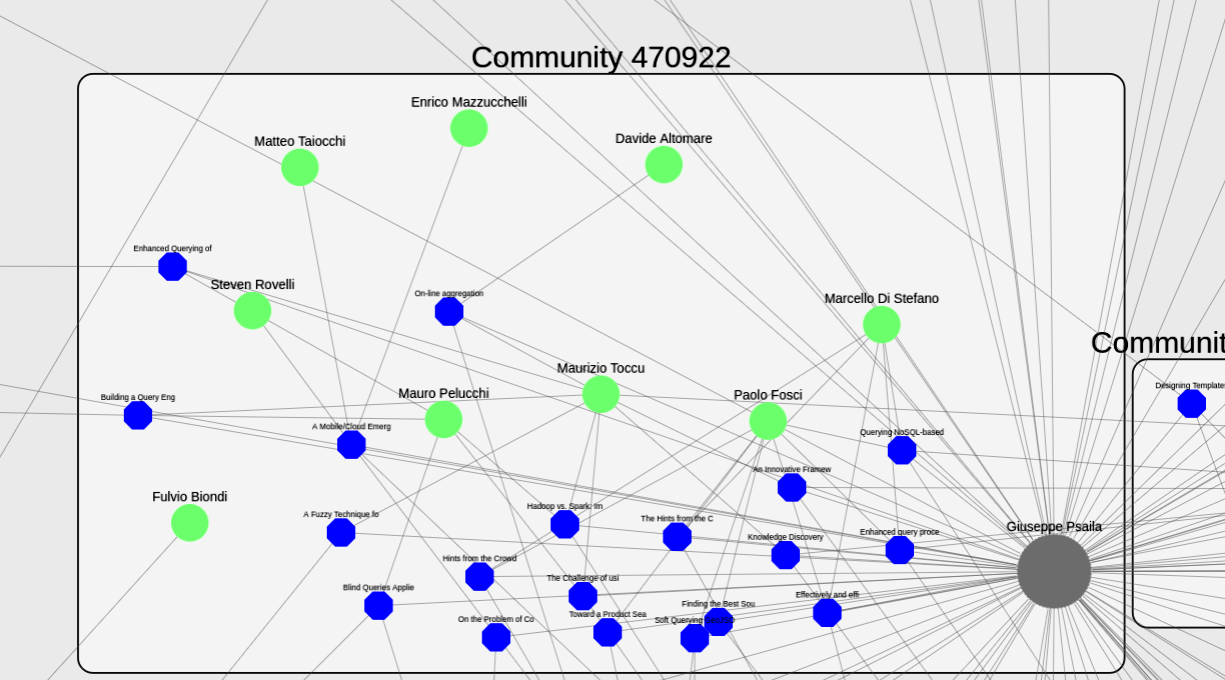
\includegraphics[%
		width=1\textwidth-4pt,%
		bgcolor=white,%
		cfbox=lightestgray % color
			  2pt % rule width
			  0pt % rule separation
			  0pt % margin
	]{images/chapter5/SnapshotLoadedGraphPsailaZoomMore.png}%
	\caption[Detailed view of the collaboration graph of prof. Psaila and of its peers, publications]{Detailed view of the collaboration graph of prof. Psaila and of its peers, publications}%
	\label{fig:SnapshotLoadedGraphPsailaZoomMore}%
\end{figure}%

Prof. Psaila is detected to be part of an academic collaboration community totally different from those of professors Gargantini and Scandurra.
Even though all three are part of the same institutional environment, that is the University of Bergamo and also part of the same faculty, departments, prof. Psaila's community is a separate one.
This has to do with fewer connections, in other words collaborations between him and the other two professor's community vertices.
Prof. Psaila collaborates with a totally different group of vertices, thus it makes sense from the point of view of the interconnections density between different groups, to be detected as part of a distinct cluster.

Something interesting to mention here is the concept of overlapping communities that will be considered in \hyperref[chapter:Conclusions]{\S\ \ref{chapter:Conclusions} - \nameref{chapter:Conclusions}} \adforn{43}\  \hyperref[section:Conclusions/Furtheravenuesofexploration]{\S\ \ref{section:Conclusions/Furtheravenuesofexploration} - \nameref{section:Conclusions/Furtheravenuesofexploration}}, specifically in \hyperref[subsection:Conclusions/Furtheravenuesofexploration/Exploringoverlappingcommunitiesdetection]{\S\ \ref{subsection:Conclusions/Furtheravenuesofexploration/Exploringoverlappingcommunitiesdetection} - \nameref{subsection:Conclusions/Furtheravenuesofexploration/Exploringoverlappingcommunitiesdetection}} on \hyperref[subsection:Conclusions/Furtheravenuesofexploration/Exploringoverlappingcommunitiesdetection]{page \pageref{subsection:Conclusions/Furtheravenuesofexploration/Exploringoverlappingcommunitiesdetection}}.
Even though prof. Psaila's community is a different one from the other two professors's, it might be interesting to consider the possibility of having overlapping parts of the different detected communities.\label{tobementionedinconclusions/Exploringoverlappingcommunitiesdetection}

In the next subsection is shown an example of a vast graph of collaboration, that of prof. Paraboschi's.

\subsection{Prof. Stefano Paraboschi's community of research collaboration} \label{subsection:Displayoftheresults/Indetailviewofthecollaborationgraph/ProfStefanoParaboschiscommunityofresearchcollaboration}
In this subsection is considered the situation of a pretty vast graph of academic collaborations that are detected as fragmented in many smaller communities.
That is the case of the graph of prof. Paraboschi, shown in \hyperref[fig:SnapshotLoadedGraphParaboschiCut]{\autoref{fig:SnapshotLoadedGraphParaboschiCut}}.

\begin{figure}[H]%
	\centering%
	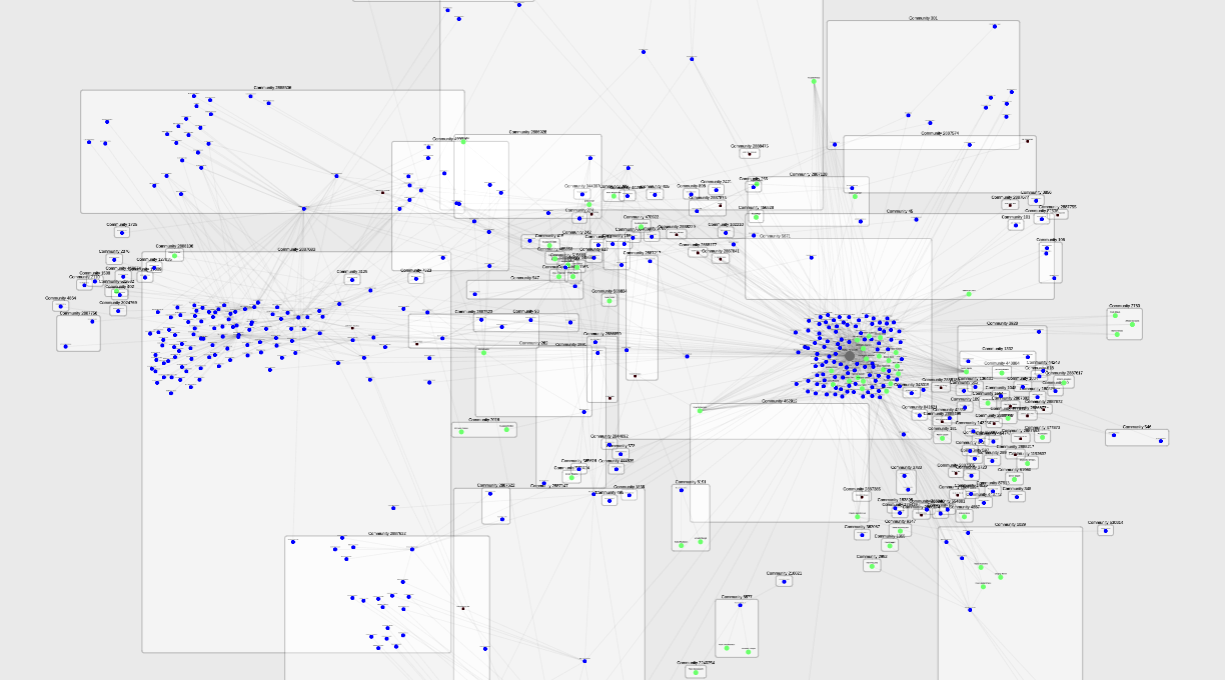
\includegraphics[%
		width=1\textwidth-4pt,%
		bgcolor=white,%
		cfbox=lightestgray % color
			  2pt % rule width
			  0pt % rule separation
			  0pt % margin
	]{images/chapter5/SnapshotLoadedGraphParaboschiCut.png}%
	\caption[Panoramic view of the collaboration graph of prof. Paraboschi]{Panoramic view of the collaboration graph of prof. Paraboschi}%
	\label{fig:SnapshotLoadedGraphParaboschiCut}%
\end{figure}%

It is visually possible to see how wide the graph is, with lots of locally sparsed groups of subcommunities.

\begin{figure}[H]%
	\centering%
	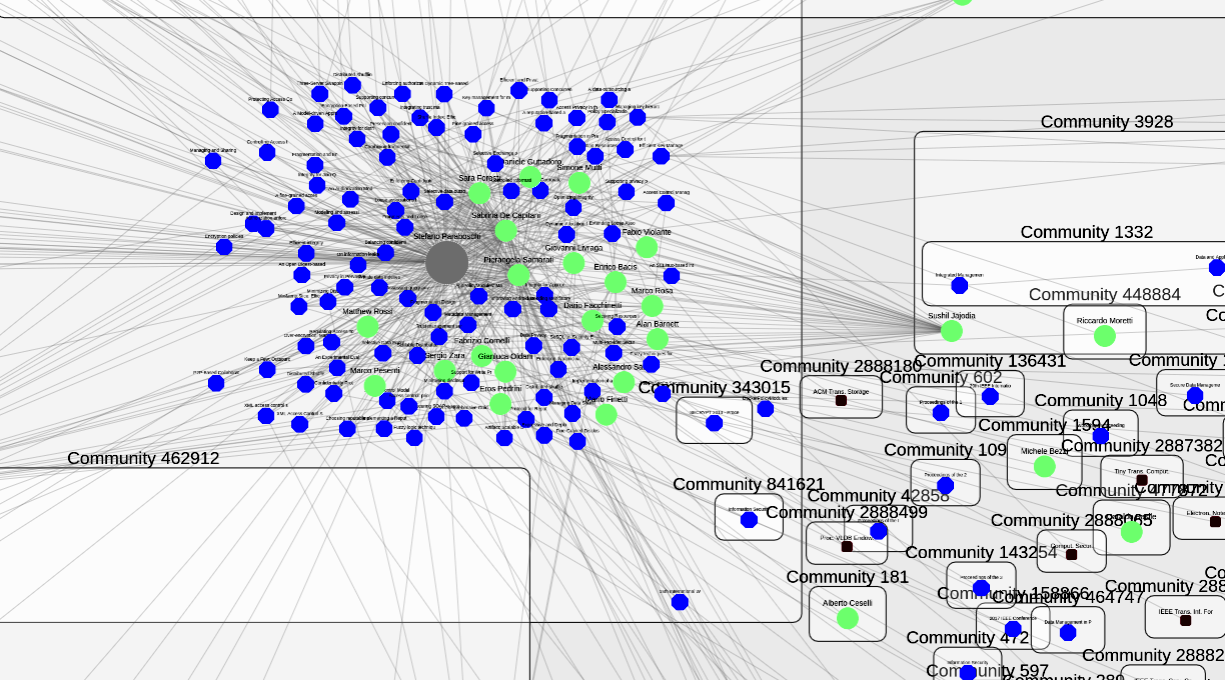
\includegraphics[%
		width=1\textwidth-4pt,%
		bgcolor=white,%
		cfbox=lightestgray % color
			  2pt % rule width
			  0pt % rule separation
			  0pt % margin
	]{images/chapter5/SnapshotLoadedGraphParaboschiZoom.png}%
	\caption[A zoom in of the collaboration graph of prof. Paraboschi]{A zoom in of the collaboration graph of prof. Paraboschi}%
	\label{fig:SnapshotLoadedGraphParaboschiZoom}%
\end{figure}%

Zooming in the graph, other features are noticeable - like for example the concentrated high density of subcommunities.
The difference in interconnection densities between groups of vertices, or between a group and some sparsely linked vertices leads to this fragmentation of detected communities. 
The relative difference of densities of links between different communities is an important parameter to consider in order to have a detection of clusters as much of a reflection of reality as possible.
This is considered in \hyperref[chapter:Conclusions]{\S\ \ref{chapter:Conclusions} - \nameref{chapter:Conclusions}} \adforn{43}\  \hyperref[section:Conclusions/Furtheravenuesofexploration]{\S\ \ref{section:Conclusions/Furtheravenuesofexploration} - \nameref{section:Conclusions/Furtheravenuesofexploration}}, specifically in \hyperref[subsection:Conclusions/Furtheravenuesofexploration/Detectionofcommunitiesandtheirhierarchyatdifferentscales]{\S\ \ref{subsection:Conclusions/Furtheravenuesofexploration/Detectionofcommunitiesandtheirhierarchyatdifferentscales} - \nameref{subsection:Conclusions/Furtheravenuesofexploration/Detectionofcommunitiesandtheirhierarchyatdifferentscales}} on \hyperref[subsection:Conclusions/Furtheravenuesofexploration/Detectionofcommunitiesandtheirhierarchyatdifferentscales]{page \pageref{subsection:Conclusions/Furtheravenuesofexploration/Detectionofcommunitiesandtheirhierarchyatdifferentscales}}.\label{tobementionedinconclusions/Detectionofcommunitiesandtheirhierarchyatdifferentscales}

In \hyperref[fig:SnapshotLoadedGraphParaboschiZoomMore]{\autoref{fig:SnapshotLoadedGraphParaboschiZoomMore}} is possible to see the highly connected vertices to the point where the area between nodes gets colored by the dense edges.

\begin{figure}[H]%
	\centering%
	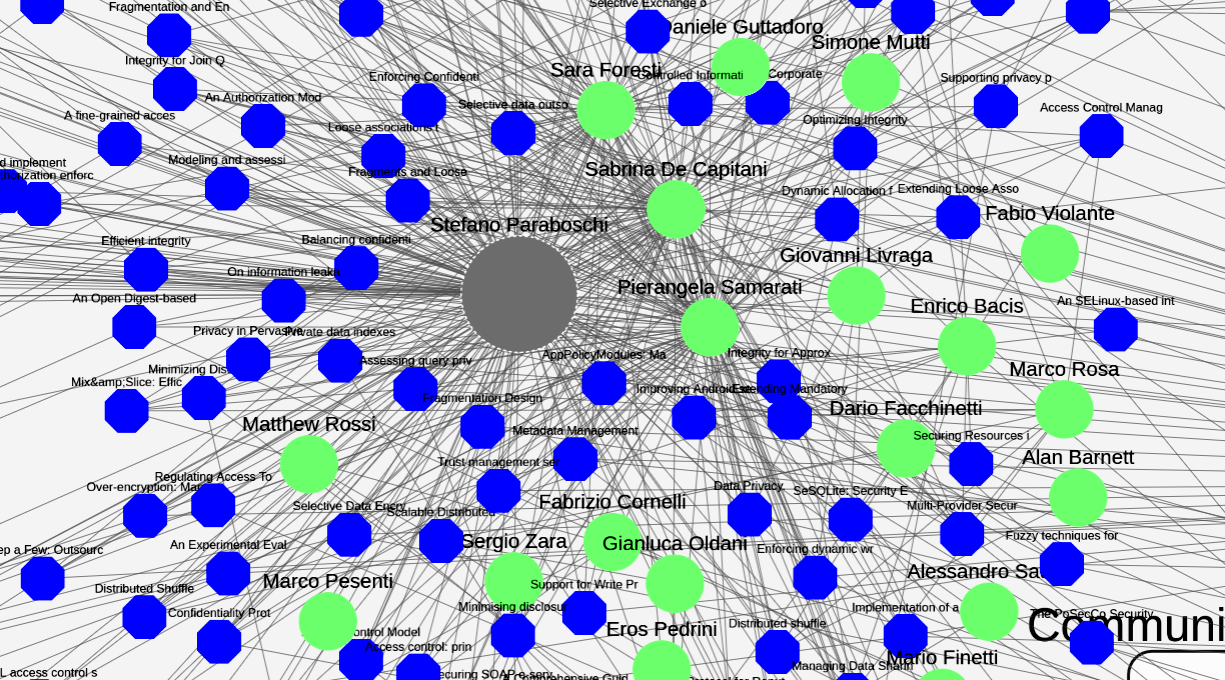
\includegraphics[%
		width=1\textwidth-4pt,%
		bgcolor=white,%
		cfbox=lightestgray % color
			  2pt % rule width
			  0pt % rule separation
			  0pt % margin
	]{images/chapter5/SnapshotLoadedGraphParaboschiZoomMore.png}%
	\caption[Detailed view of the collaboration graph of prof. Paraboschi and of its peers, publications]{Detailed view of the collaboration graph of prof. Paraboschi and of its peers, publications}%
	\label{fig:SnapshotLoadedGraphParaboschiZoomMore}%
\end{figure}%

In the next two subsections are shown graphs of academic collaborations build around a vertex that is not an author, such as for example having a start node set as a journal or as an institution.

\subsection{Graph of the community of the \textit{Statistical Methods \& Applications} journal and prof. Alessandro Fas\-sò no\-de} \label{subsection:Displayoftheresults/Indetailviewofthecollaborationgraph/GraphofthecommunityoftheStatisticalMethodsApplicationsjournalandprofAlessandroFassonode}
In this subsection is shown a graph of academic collaborations formed around a journal, \textit{Statistical Methods \& Applications} - that is the journal of the \textit{Italian Statistical Society}.\sfcite{ItalianStatisticalSociety2021}.

\hyperref[fig:SnapshotLoadedGraphJournal]{\autoref{fig:SnapshotLoadedGraphJournal}} and \hyperref[fig:SnapshotLoadedGraphJournalZoom]{\autoref{fig:SnapshotLoadedGraphJournalZoom}} offer a lot of graphically accessible information for an interested user.
The graph is associated to only one focal input, that is the name of the journal.
The same can be done with a series\footnote{\url{https://en.wikipedia.org/wiki/Serial_(publishing)}} for example.

\begin{figure}[H]%
	\centering%
	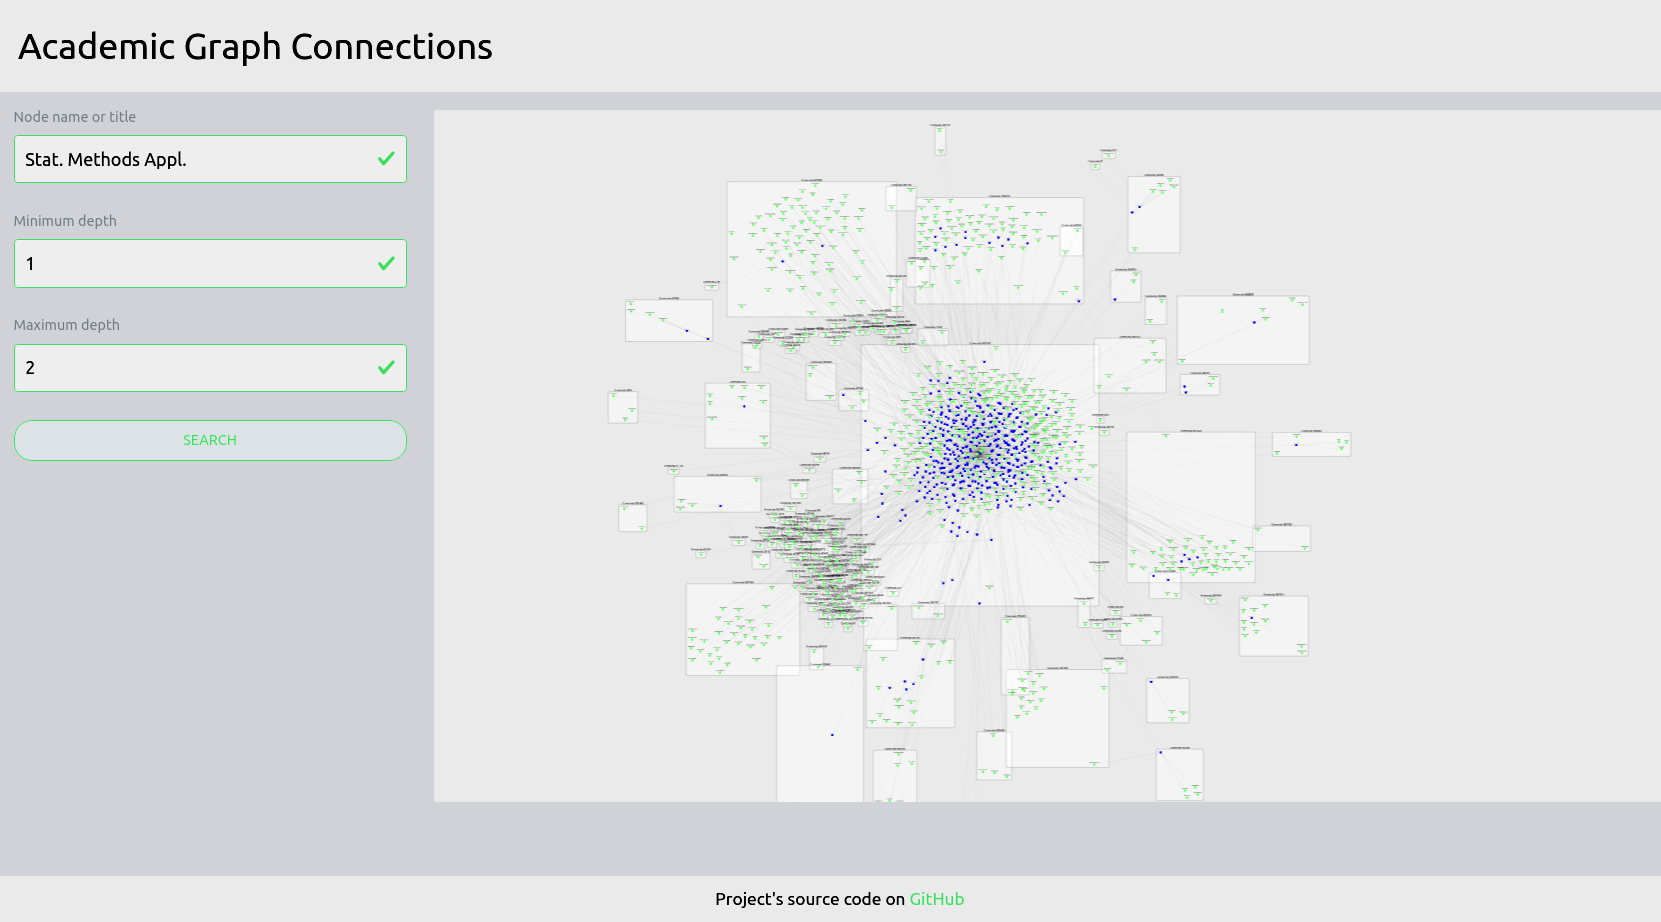
\includegraphics[%
		width=1\textwidth-4pt,%
		bgcolor=white,%
		cfbox=lightestgray % color
			  2pt % rule width
			  0pt % rule separation
			  0pt % margin
	]{images/chapter5/SnapshotLoadedGraphJournal.png}%
	\caption[Searching for the collaboration communities built around \textit{Statistical Methods \& Applications} journal]{Searching for the collaboration communities built around \textit{Statistical Methods \& Applications journal}}%
	\label{fig:SnapshotLoadedGraphJournal}%
\end{figure}%

\begin{figure}[H]%
	\centering%
	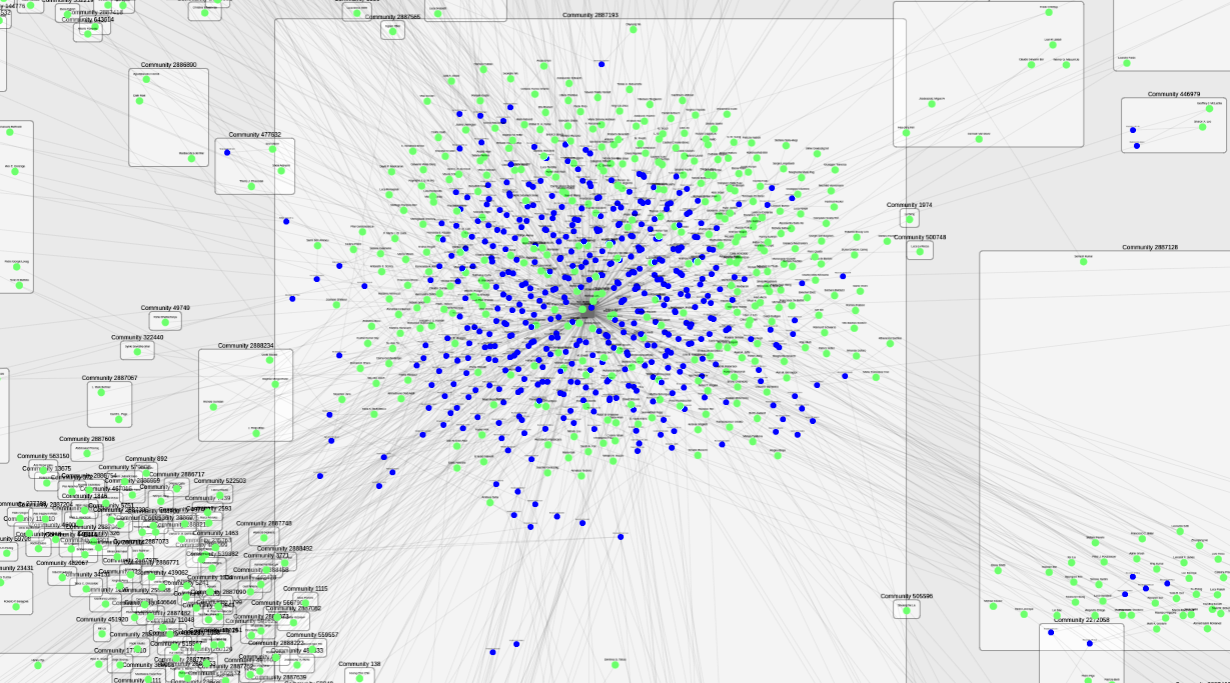
\includegraphics[%
		width=1\textwidth-4pt,%
		bgcolor=white,%
		cfbox=lightestgray % color
			  2pt % rule width
			  0pt % rule separation
			  0pt % margin
	]{images/chapter5/SnapshotLoadedGraphJournalZoom.png}%
	\caption[Zoomed in view of the graph of collaboration communities built around Statistical Methods \& Applications journal]{Zoomed in view of the graph of collaboration communities built around Statistical Methods \& Applications journal}%
	\label{fig:SnapshotLoadedGraphJournalZoom}%
\end{figure}%

At the bottom part of \hyperref[fig:SnapshotLoadedGraphJournalZoomMoreFasso]{\autoref{fig:SnapshotLoadedGraphJournalZoomMoreFasso}}, in the middle is found the professor of statistics at the University of Bergamo, Alessandro Fassò - part of the enormous academic collaboration community of researchers who publish in \textit{Statistical Methods \& Applications journal}.

In the next subsection is presented the graph of the communities affiliated to the most prestigious computer science university in Europe, ETH Zurich, Switzerland.

\begin{figure}[H]%
	\centering%
	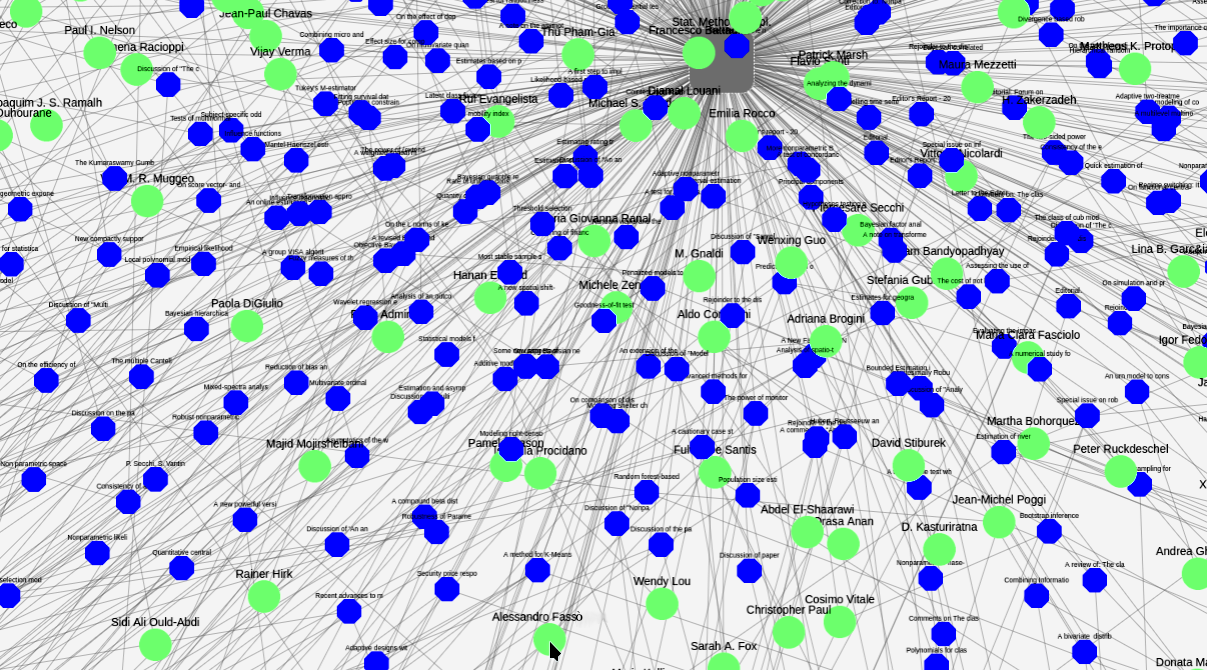
\includegraphics[%
		width=1\textwidth-4pt,%
		bgcolor=white,%
		cfbox=lightestgray % color
			  2pt % rule width
			  0pt % rule separation
			  0pt % margin
	]{images/chapter5/SnapshotLoadedGraphJournalZoomMoreFasso.png}%
	\caption[Detailed view of the graph of communities of Statistical Methods \& Applications journal and prof. Alessandro Fassò node]{Detailed view of the graph of communties of Statistical Methods \& Applications journal and prof. Alessandro Fassò node}%
	\label{fig:SnapshotLoadedGraphJournalZoomMoreFasso}%
\end{figure}%

\subsection{Graph of researchers affiliated to ETH Zurich} \label{subsection:Displayoftheresults/Indetailviewofthecollaborationgraph/GraphofresearchersaffiliatedtoETHZurich}
A special case of graphs regarding academic collaboration communities are the ones built around universities, schools and research institutions in general. In this last subsection are shown two graphs.
In \hyperref[fig:SnapshotLoadedGraphETHZurichSwitzerland11]{\autoref{fig:SnapshotLoadedGraphETHZurichSwitzerland11}} is presented a maximum 1 hop graph of the communities in ETH Zurich, Switzerland. It shows only the researchers directly affiliated to that institution.

\begin{figure}[H]%
	\centering%
	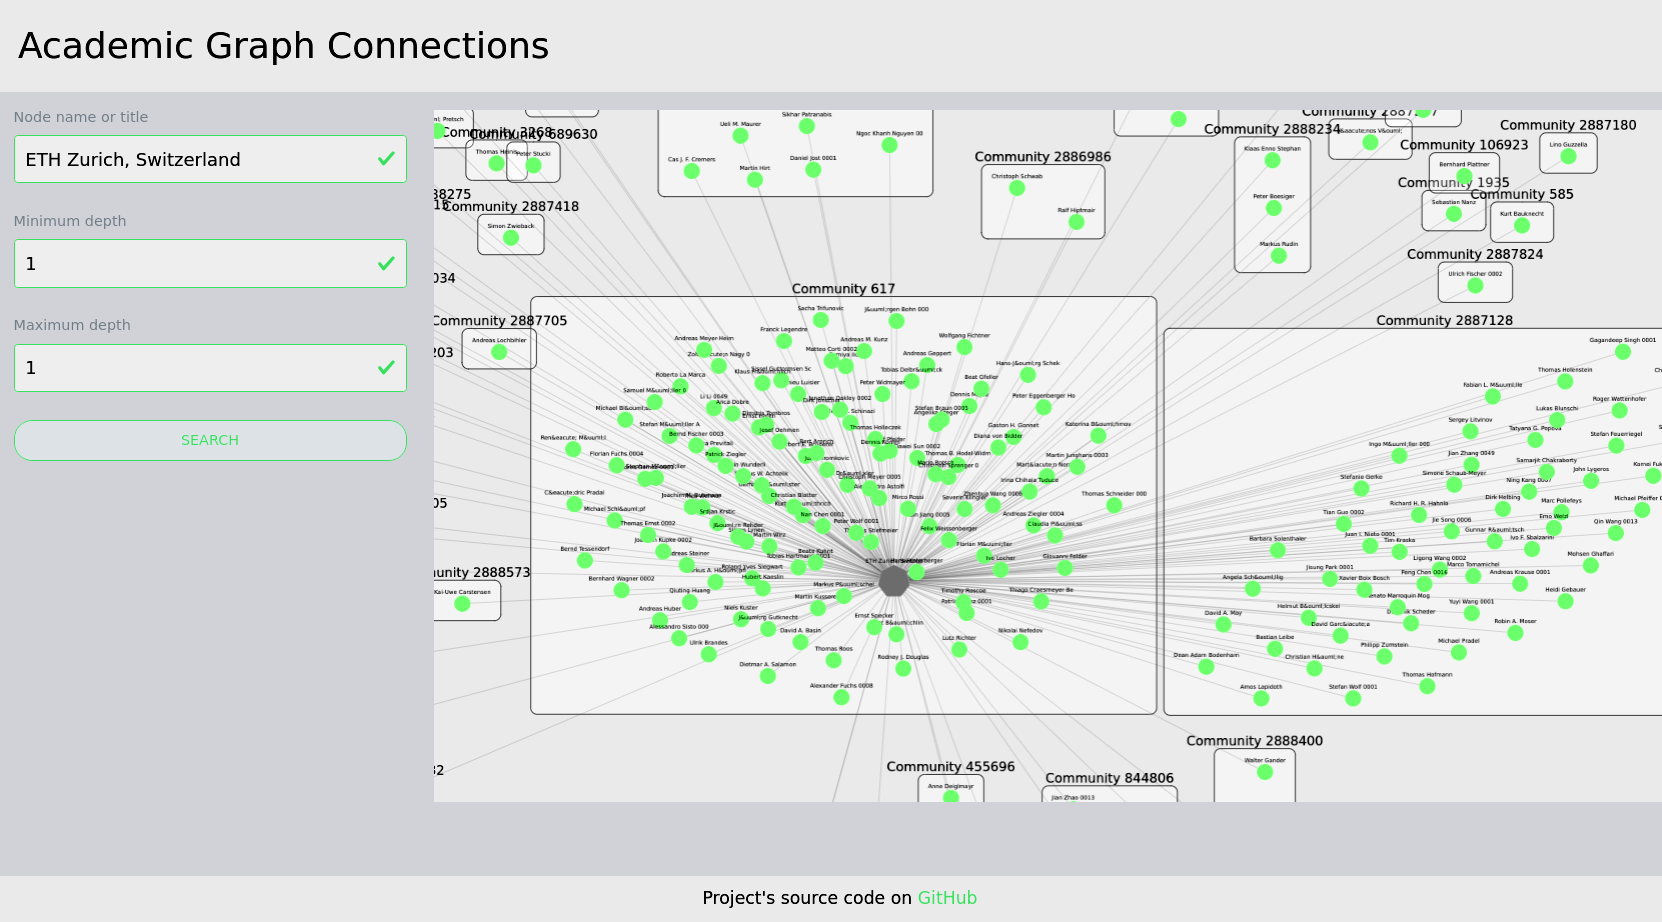
\includegraphics[%
		width=1\textwidth-4pt,%
		bgcolor=white,%
		cfbox=lightestgray % color
			  2pt % rule width
			  0pt % rule separation
			  0pt % margin
	]{images/chapter5/SnapshotLoadedGraphETHZurichSwitzerland11.png}%
	\caption[Detailed view of the graph of the authors of the academic communities at ETH Zurich, Switzerland]{Detailed view of the graph of the authors of the academic communities at ETH Zurich, Switzerland}%
	\label{fig:SnapshotLoadedGraphETHZurichSwitzerland11}%
\end{figure}%

Whereas in \hyperref[fig:SnapshotLoadedGraphETHZurichSwitzerland11]{\autoref{fig:SnapshotLoadedGraphETHZurichSwitzerland11}} is presented a maximum 2 hops graph of the colalboration communities in ETH Zurich.
Since the maximum depth is set to 2, the publications of the researchers (the dark blue nodes) are also shown as part of the communities. 

\begin{figure}[H]%
	\centering%
	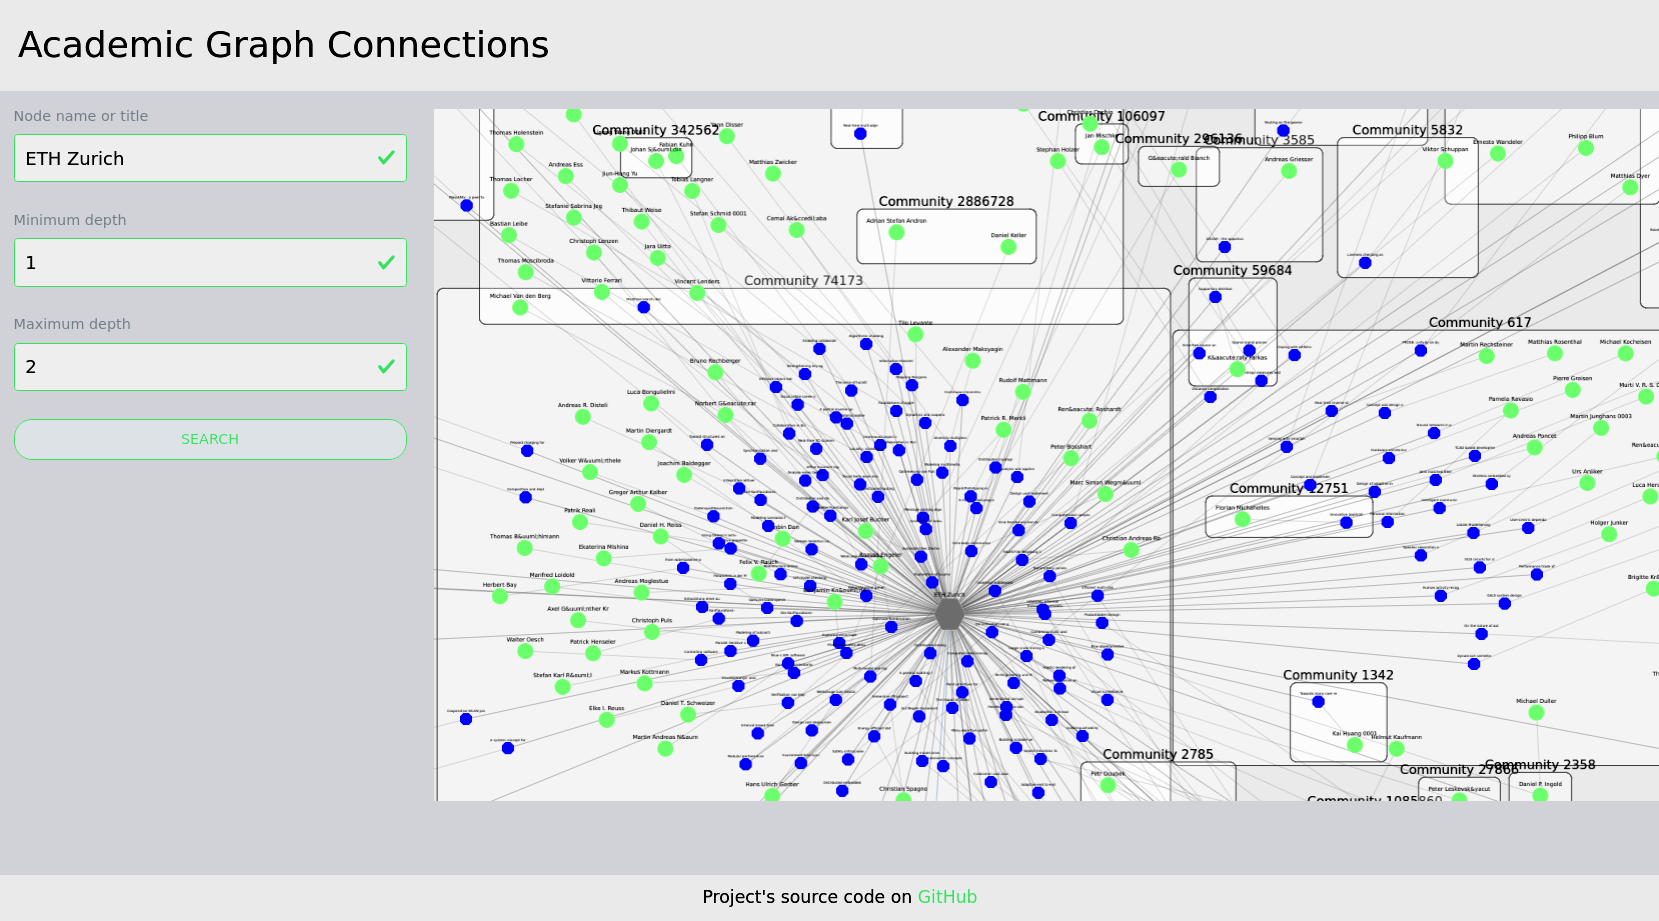
\includegraphics[%
		width=1\textwidth-4pt,%
		bgcolor=white,%
		cfbox=lightestgray % color
			  2pt % rule width
			  0pt % rule separation
			  0pt % margin
	]{images/chapter5/SnapshotLoadedGraphETHZurich12.png}%
	\caption[Detailed view of the graph of academic collaborations at ETH Zurich]{Detailed view of the graph of academic collaborations at ETH Zurich}%
	\label{fig:SnapshotLoadedGraphETHZurich12}%
\end{figure}%

For more exploration, visit \citeurl{adomainthatrocks2021}.\sfcite{adomainthatrocks2021}

\newpage
\thispagestyle{empty}
